
%(BEGIN_QUESTION)
% Copyright 2015, Tony R. Kuphaldt, released under the Creative Commons Attribution License (v 1.0)
% This means you may do almost anything with this work of mine, so long as you give me proper credit

Calculate the amount of current through $R_1$ in this series-parallel circuit, as well as the voltage between points D and F.  There is no need to specify the direction of the current or the polarity of the voltage.  Assume all resistors are 1 k$\Omega$ in resistance:

$$\includegraphics[width=15.5cm]{i00204x01.eps}$$

$I_{R1}$ = 

\vskip 10pt

$V_{DF}$ = 

\vskip 10pt

\underbar{file i00204}
%(END_QUESTION)





%(BEGIN_ANSWER)

$I_{R1}$ = 14.4 mA

\vskip 10pt

$V_{DF}$ = 4.8 V

%(END_ANSWER)





%(BEGIN_NOTES)

{\bf This question is intended for exams only and not worksheets!}.

%(END_NOTES)


